\documentclass[UTF8]{ctexart}
% \usepackage{newtxtext}
\usepackage[dvipsnames,svgnames,x11names]{xcolor} %颜色宏包
\usepackage{lipsum} %生成一段文字
\usepackage[dvipsnames,svgnames]{xcolor}
\usepackage[strict]{changepage} % 提供一个 adjustwidth 环境
\usepackage{framed} % 实现方框效果
% 数学宏包
\usepackage{amsmath}
\usepackage{amssymb}
\usepackage{bbm} %使用\mathbbm{}
% 插入图片
% % https://www.latex4technics.com/?note=44HZ

% 用于定义插入封面图片的命令
% 用法:\coverimage{图片文件名}{图片宽度}
\newcommand{\coverimage}[2][]{
    \begin{figure}[H]
        \centering
        \includegraphics[width=#2]{#1}
    \end{figure}
}
% 用于定义插入图片的命令
% 用法:\insertimage{图片文件名}{图片宽度}{图片标题}
\newcommand{\insertimage}[3]{
    \begin{figure}[H]
        \centering
        \includegraphics[width=#2]{#1}
        \caption{#3}
    \end{figure}
}
% 用于定义插入图片的命令
% 用法:\insertimage{图片文件名}{图片宽度}{图片标题}
\newcommand{\insertimageleft}[3]{
    \begin{figure}[H]
        \flushleft
        \includegraphics[width=#2]{#1}
        \caption{#3}
    \end{figure}
}
% 用于定义插入图片的命令
% 用法:\insertimage{图片文件名}{图片宽度}{图片标题}
\newcommand{\insertimageright}[3]{
    \begin{figure}[H]
        \flushright
        \includegraphics[width=#2]{#1}
        \caption{#3}
    \end{figure}
}


\usepackage{graphicx} %插入图片
\usepackage{float} %设置图片浮动位置
\usepackage{subfigure} %插入多图时用子图显示
\graphicspath{{./pic/},{./pic/decoration/}} %存放图片的文件夹
\DeclareGraphicsExtensions{.pdf,.jpeg,.png,.jpg}

% ------------------** 字体 **------------------
\usepackage{type1cm} %设置字号
% ------------------** 外部设置 **------------------
% 文本框样式
% ---
% Module Name: textbox.tex
% description: 文本框底纹配置文件
% ---
\usepackage{tcolorbox}
% 颜色定义
\definecolor{formalshade}{rgb}{0.95,0.95,1}
\definecolor{greenshade}{rgb}{0.90,0.99,0.91} %绿色文本框,竖线颜色设为 Green
\definecolor{redshade}{rgb}{1.00,0.90,0.90} %红色文本框,竖线颜色设为 LightCoral
\definecolor{brownshade}{rgb}{0.99,0.97,0.93} %莫兰迪棕色,竖线颜色设为 BurlyWood
% 注意行末需要把空格注释掉,不然画出来的方框会有空白竖线
%蓝紫色
\newenvironment{Chinese Note}{%
	\def\FrameCommand{%
		\hspace{1pt}%
		{\color{DarkBlue}\vrule width 2pt}%
		{\color{formalshade}\vrule width 4pt}%
		\colorbox{formalshade}%
	}%
	\MakeFramed{\advance\hsize-\width\FrameRestore}%
	\noindent\hspace{-4.55pt}% disable indenting first paragraph
	\begin{adjustwidth}{}{7pt}%
		\vspace{2pt}\vspace{2pt}%
	}
	{%
		\vspace{2pt}\end{adjustwidth}\endMakeFramed%
}
%棕色
\newenvironment{English Note}{%
	\def\FrameCommand{%
		\hspace{1pt}%
		{\color{BurlyWood}\vrule width 2pt}%
		{\color{brownshade}\vrule width 4pt}%
		\colorbox{brownshade}%
	}%
	\MakeFramed{\advance\hsize-\width\FrameRestore}%
	\noindent\hspace{-4.55pt}% disable indenting first paragraph
	\begin{adjustwidth}{}{7pt}%
		\vspace{2pt}\vspace{2pt}%
	}
	{%
		\vspace{2pt}\end{adjustwidth}\endMakeFramed%
}

% ------------------** 页面布局 **------------------
\usepackage{geometry} %页面设置
% a4纸; 水平、竖直均居中
\geometry{a4paper,centering,scale=0.9}
\usepackage{fancyhdr}
\pagestyle{fancy}
\setlength{\headheight}{12.7pt} %设置页眉高度,不设就会有 warning
% style
%   empty - 页眉和页脚都没有
\lhead{}
\chead{Mind Map} 
\rhead{by Feynman's Little Brother}
\lfoot{}
\cfoot{What one fool can understand, another can.}
\rfoot{}
% \thepage - 页码
% \today - 今日日期
\renewcommand\headrulewidth{2pt} %页眉线宽度
\renewcommand\footrulewidth{2pt} %页脚线宽度
% 标题设置
\usepackage[raggedright]{titlesec}
% \titleformat{\section}{\Large\bfseries}{Section \thesection}{1em}{} %英文标题
\titleformat{\section}{\Large\bfseries}{第 \thesection\ 节}{1em}{} %中文标题
% ------------------** 定理设置 **------------------
\newtheorem{theorem1}{定理}
\newtheorem{example}{例}

% ------------------** 封面页设置 **-------------------
\usepackage{tikz}
\usepackage{fancyhdr}

\fancypagestyle{coverpage}{
    \fancyhf{} % clear all header and footer fields
    \renewcommand{\headrulewidth}{0pt} % remove the header rule
    \fancyhead[C]{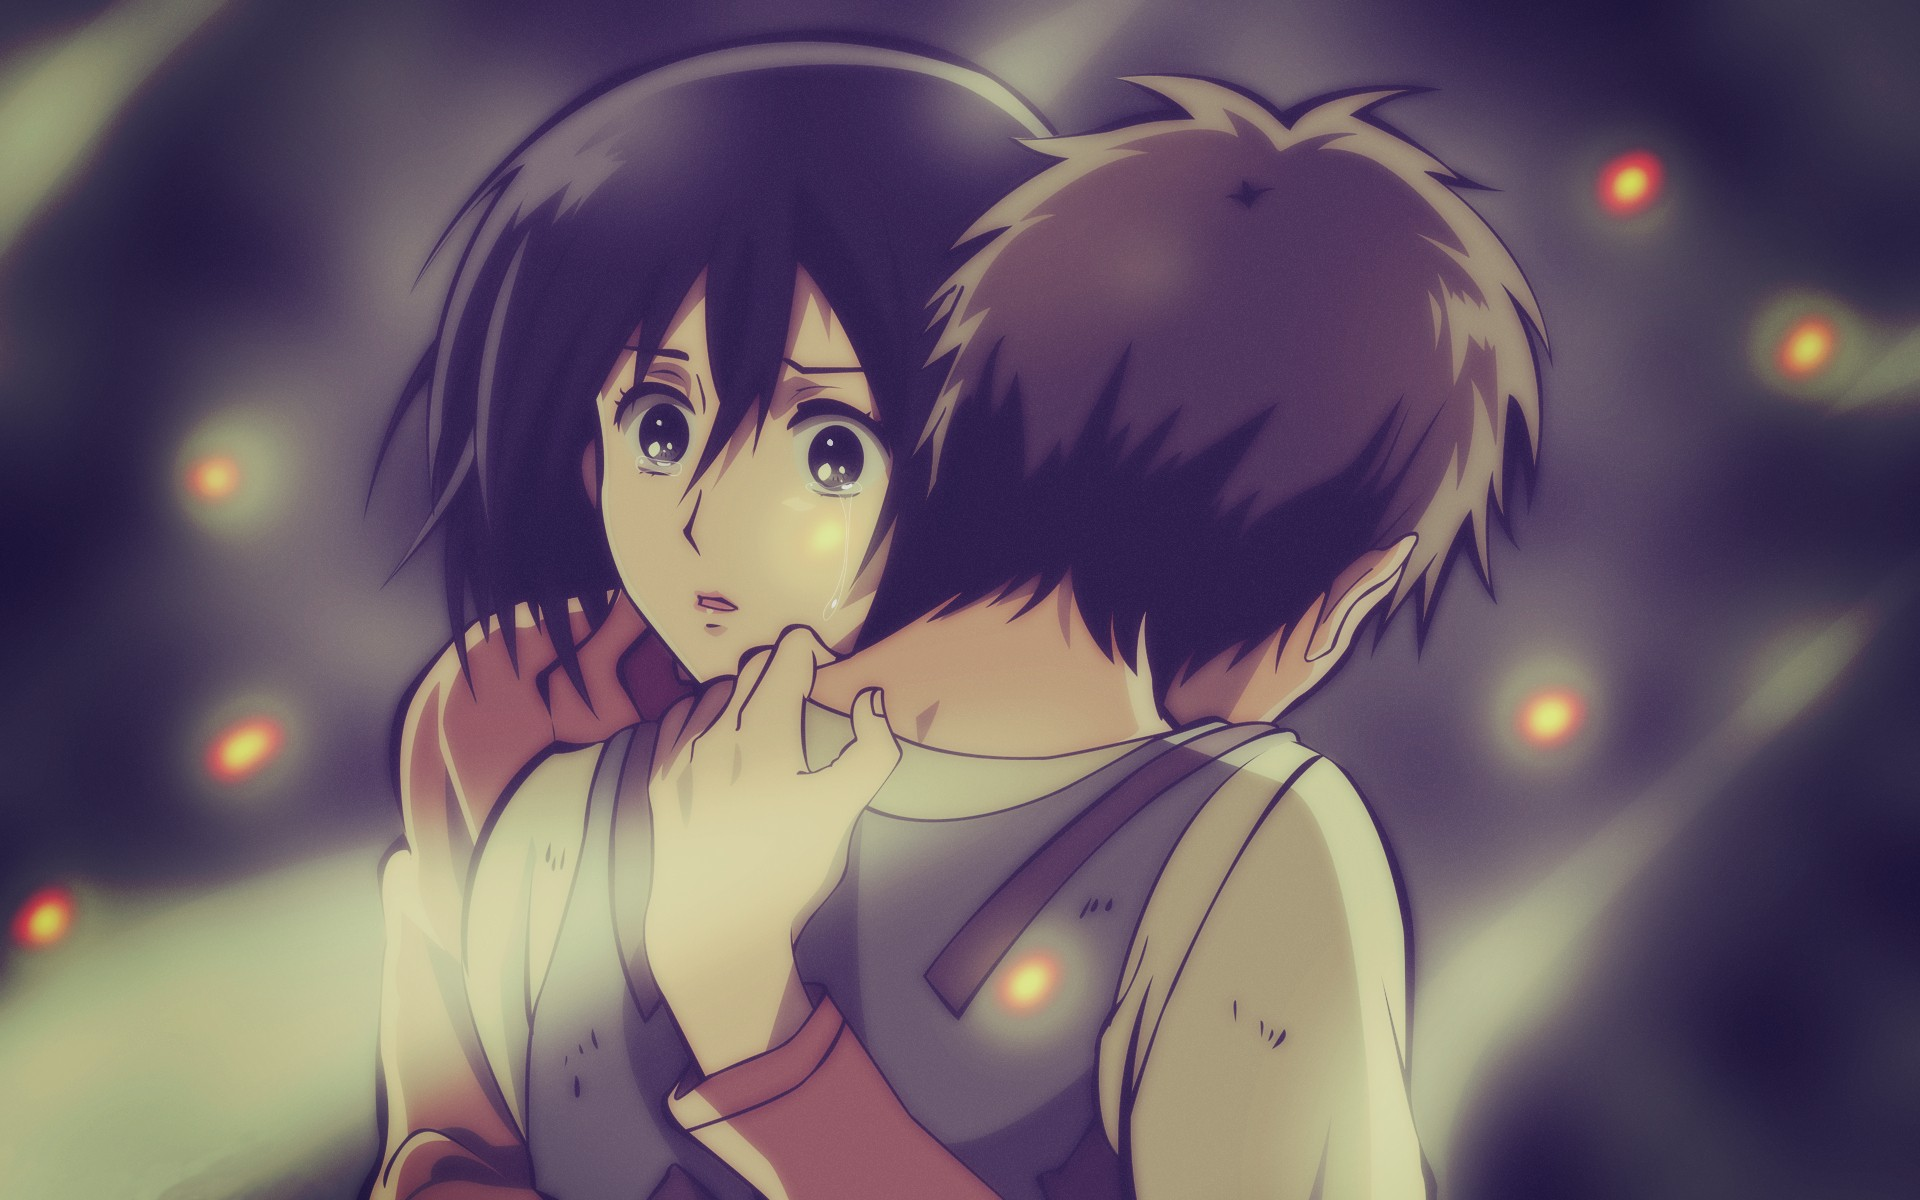
\includegraphics[width=1\paperwidth,height=0.4\paperwidth,trim=500 50 50 50,clip]{cover}} % add the cover page image to the header
}
% ------------------** 正文 **-------------------
\title{\fontsize{40pt}{80pt} $\mathbbm{Advance Algebra}$}
\author{\textcolor{ForestGreen}{Feynman's Little Brother}}

\begin{document}
% \thispagestyle{fancy} %让首页也有页眉

% ---------- 正文部分 ----------
\section{常微分方程}
    \subsection{初等积分法}
($\star$)
\subsection{线性方程}
\begin{enumerate}
    \item 存在性与唯一性
    \begin{enumerate}
        \item ($\star$)假设$A(t)$是区间$[\alpha, \beta]$上的连续矩阵函数, $f(t)$是区间$[\alpha, \beta]$上的连续列向量函数, 
        则初值问题$\frac{d}{dt}x=Ax+f(t), x(t_0)=x^0$在区间$[\alpha, \beta]$上存在唯一解
        \item 齐次方程
    \end{enumerate}
\end{enumerate}
\subsection{常系数线性方程}
线性微分方程求解的关键就在通解的求得, 而常系数下通解有办法求得
\begin{enumerate}
    \item 齐次通解 -- Euler待定指数法\\
    证明这些解线性无关($\star$)
    \begin{enumerate}
        \item 列出特征方程$P(\lambda)=0$,求出特征根
        \item (1) $P(\lambda)=0$有n个互异实根
        \item (2) $P(\lambda)=0$有r个互异实根
        \item (3) $P(\lambda)=0$有r个互异实根和l对共轭互异复根
    \end{enumerate}
    \item 非齐次特解 -- 算子法\\
    算子解法比常数变易公式更简便些
    \begin{enumerate}
        \item 解析展开法
        \item 代换法
        \item 二项式法
    \end{enumerate}
    \item 常系数线性方程组
    根据矩阵$A$的特征值得到方程的通解
    \begin{enumerate}
        \item ($\star$) 若A有n个互异实特征根, 则方程组$\frac{d}{dt}x=Ax$有基本解组$e^{\lambda_{1}t}c_1, e^{\lambda_{2}t}c_2, \cdots, e^{\lambda_{n}t}c_n$,其中$c_i$为$\lambda_i$的特征向量
        \item 矩阵指数函数$e^{tA}$ (一定收敛)
        \item ($\star$) 齐次方程组$\frac{d}{dt}x =Ax$有标准解矩阵$e^{tA}$, 
        非齐次方程$\frac{d}{dt}x=Ax+f(t)$的通解为$x=e^{tA}c + \int_{t_0}^{t} e^{(t-s)A}f(s)ds$
        \item 标准解矩阵的初等表达: 把$e^{tA}$转换成有限和的形式算出来
    \end{enumerate}
    \item 应用:机械振动
    \begin{enumerate}
        \item 无阻尼自由振动 $\ddot{x}+\omega^2 x=0$
        \item 有阻尼自由振动 $\ddot{x}+2\delta \dot{x}+\omega^2 x=0$
        \item 无阻尼强迫振动 $\ddot{x}+\omega^2 x = \frac{F_0}{m}\cos pt$
        \item 有阻尼强迫振动 $\ddot{x}+2\delta \dot{x}+\omega^2 x = \frac{F_0}{m}\cos pt$
    \end{enumerate}
\end{enumerate}

\subsection{一般理论}
\begin{enumerate}
    \item Picard存在唯一性定理
    \begin{itemize}
        \item $\dot{x}=f(t,x), x(t_0)=x_0$,其中$f(t,x)$连续且满足Lipschiz条件,
        则初值问题在区间$|t-t_0|\leq h$存在唯一解
        \item 构造Picard序列 -- 求近似解 $\varphi_{n}(t) = x_0 + \int_{t_0}^{t}f(\tau , \varphi_{n-1}(\tau))d\tau$
        \item Picard序列误差估计 $|\varphi_{n}(t) - \varphi(t)| \leq \frac{ML^{n}}{(n+1)!}h^{n+1}$
    \end{itemize}
    \item Peano存在性定理
    \begin{itemize}
        \item \textbf{Ascoli-Arzela定理} $[\alpha, \beta]$上的一致有界且等度连续的函数列${f_k(t)}$有一致收敛的子序列
        \item $\dot{x}=f(t,x), x(t_0)=x_0$,其中$f(t,x)$连续,
        则初值问题在区间$|t-t_0|\leq h$有至少一个解 (没有Lipschiz条件,解仍存在但是不唯一)
        \item 构造Eule折线, 证明其是$\epsilon$-逼近解
    \end{itemize}
    \item 解的延拓
    \begin{itemize}
        \item 饱和解的存在区间为开区间
        \item \textbf{解的延拓定理} G为$\mathbb{R}^2$上的开区间, $f(t,x)$在G内连续,
        则对$\dot{x}=f(t,x)$的任一饱和解$\varphi(t)$必能到达G的边界
        \item 找一个比函数连续区域更小的区域,得到矛盾
    \end{itemize}
    \item 微分不等式与比较定理
    \begin{itemize}
        \item ($\star$) \textbf{Gronwall不等式} x(t), f(t)在$[t_0, t_1]$上连续,$f(t)\geq 0$, 若$x(t)\leq g + \int_{t_0}^{t}f(s)x(s)ds$, 则$x(t)\leq g\exp(\int_{t_0}^{t}f(s)ds)$
        \item \textbf{推广Gronwall不等式} x(t), f(t), g(t)在$[t_0, t_1]$上连续,$f(t)\geq 0$, 若$x(t)\leq g(t) + \int_{t_0}^{t}f(s)x(s)ds$, 则$x(t)\leq g(t) + \int_{t_0}^{t}f(\tau)g(\tau)e^{\int_{\tau}^{t}f(s)ds}d\tau$
        \item ($\star$) \textbf{第一比较定理}, 证明时注意描述
        \item ($\star$) 最大解和最小解的存在性和唯一性, 可延拓性, 证明时构造递减序列
        \item ($\star$) \textbf{第二比较定理}, 证明时构造递减序列
    \end{itemize}
    \item 解对初值和参数的依赖
    \item 微分方程数值解
\end{enumerate}
\subsection{定性理论初步}
\begin{enumerate}
    \item 动力系统概念
    \item Lyapunov稳定性
    \item Lyapunov直接法
    \item 平面平衡点分析
    \item 周期轨道与Poincare映射
    \item 平面Hamilton系统
\end{enumerate}

    \newpage

\section{系统模型}
    \subsection{频率响应分析}
\begin{enumerate}
    \item 传递函数和Bode图之间的转换
    \begin{itemize}
        \item 典型环节
        \item 转角频率
        \item 谐振峰值
    \end{itemize}
    \item 静态误差常数
    \item Nyquist图和Nyquist稳定性判据
    \item 相对稳定性
    \begin{itemize}
        \item 增益交界频率, 相位裕量
        \item 相位交界频率, 增益裕量
        \item 谐振频率, 谐振峰值, 带宽
    \end{itemize}
    \item 串联校正
    \begin{itemize}
        \item 超前校正
        \begin{itemize}
            \item 题型1: 
        \end{itemize}
        \item 滞后校正
        \item 滞后-超前校正
    \end{itemize}
\end{enumerate}
    \newpage
\end{document}